\documentclass[svgnames,14pt]{beamer}
\usepackage[utf8]{inputenc}
\usepackage{caption}
\usepackage{graphicx}
\usepackage{xcolor}
\usepackage{wrapfig}
\usepackage{algorithm}
\usepackage{algpseudocode}
\title{The 3D Organization of Chromatin Explains Evolutionary Fragile Genomic Regions by \\ \vspace{12pt} \normalsize{Camille Berthelot, Matthieu Muffato, \\ Judith Abecassis and Hugues Roest Crollius} }
\author{Speaker: Ilia Minkin}
\institute{}
\algnotext{EndFor}
\algnotext{EndIf}
\algnotext{EndWhile}
\setbeamertemplate{footline}[frame number]
\setbeamertemplate{navigation symbols}{}
\setbeamertemplate{caption}[numbered]
\captionsetup[figure]{labelformat=empty}

\begin{document}

\date{24th April 2015}
\maketitle

\begin{frame}
\frametitle{Two types of genome alterations}

1. Small point mutations:

{\vspace{12pt} \Large \color{Blue}
ACTTG\\
A{\color{Red}G}T--\hspace{2.7pt}G
\vspace{12pt}}

\pause
2. Large rearrangements:
\begin{itemize}
\item Inversions
\item Transpositions
\item Fusions
\item ...
\end{itemize}
\end{frame}

\begin{frame}
\frametitle{Genome Rearrangements}
\begin{figure}
	\centering
	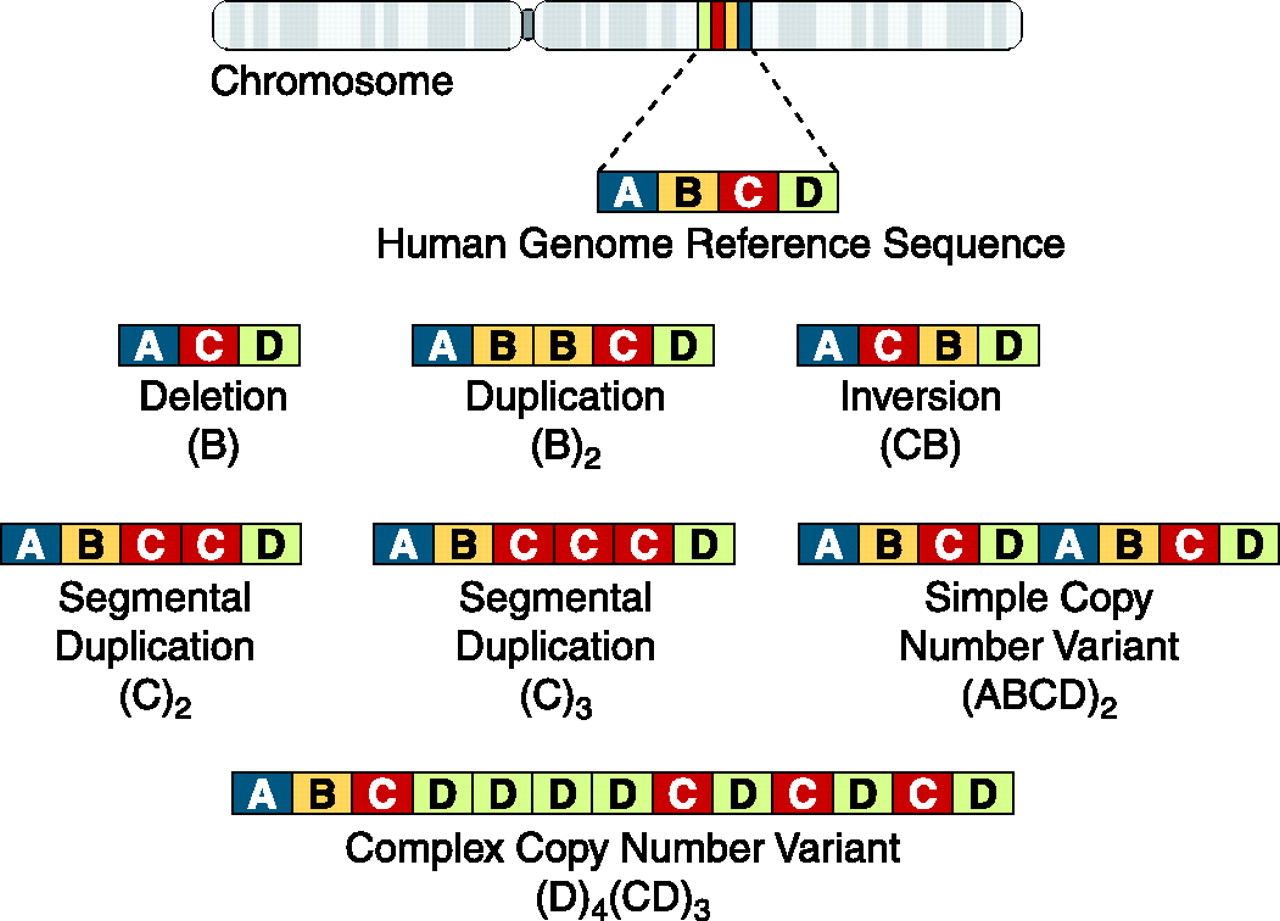
\includegraphics[scale = 0.30]{BasicRearr.jpg}
\caption{Source: \textit{Dierssen et al, 2009}}
\end{figure}
\end{frame}

\begin{frame}
\frametitle{Motivation}
Rearrangements:
\begin{itemize}
\item Are a major driving force in evolution
\item Play large role in diseases (e.g. cancer)
\end{itemize}
Known mechanisms:
\begin{itemize}
\item Non-homologous end joining
\item Non-allelic homologous recombination
\item Replication fork stalling
\item ...
\end{itemize}
\end{frame}

\begin{frame}
\frametitle{The Big Question}
Are rearrangements more likely to happen in one parts of a genome than the others?
\pause

\vspace{12pt}
Two hypotheses:
\begin{enumerate}
\item Rearrangement rates are the same for all parts of a genome
\item Some regions are more likely to be disrupted than the others
\end{enumerate}
\end{frame}

\begin{frame}
\frametitle{A Short Survey}
In 1984, Nadeau and Taylor presented first arguments in favor of random breakage

\pause
\vspace{12pt}
Pevzner and Tesler in 2003 showed evidence of fragile regions

\pause
\vspace{12pt}
Ma et al., 2006 argued for random model with higher resolution analysis of rearrangements 
\end{frame}

\begin{frame}
\frametitle{The Study}
Two questions:
\begin{itemize}
\item Do fragile regions exist?
\item If they do, what is the cause of fragility?
\end{itemize}

\vspace{12pt}
A note: fragility is not "physical", it only means higher possibility of rearrangements
\end{frame}

\begin{frame}
\frametitle{Genomes Representations}
Genomes are sequences of gene markers that are unbreakable:
\begin{figure}
	\centering
	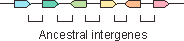
\includegraphics[scale = 2.20]{Intergenes.pdf}
\end{figure}
\pause
\vspace{12pt}
Here red dashes are breakpoints:
\begin{figure}
	\centering
	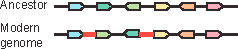
\includegraphics[scale = 2.20]{Breakpoint.pdf}
\end{figure}
\end{frame}

\begin{frame}
\frametitle{Methodology}
Boreoeutheria: the last common ancestor of primates, rodents, and laurasiatherians

\vspace{12pt}
There are representations of  human, mouse, dog, cow and horse genomes as gene sequences

\vspace{12pt}
We can reconstruct the gene order of Boreoeutheria

\vspace{12pt}
Idea: if two genes are adjacent modern genomes, the adjacency is likely to be in the ancestor
\end{frame}

\begin{frame}
\frametitle{Methodology}
\vspace{12pt}
Stages of the study:
\begin{itemize}
\item Reconstruct gene order of Boreoeutheria
\item Annotate ancestral intergenes
\item Identify breakpoints w.r.t. human, mouse, dog, cow and horse
\item Count breakpoints per intergene
\item Do regression of breakpoint counts
\end{itemize}
\end{frame}

\begin{frame}
\frametitle{The Phylogenetic Tree}
\begin{figure}
	\centering
	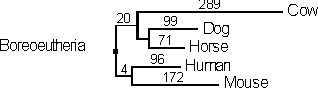
\includegraphics[scale = 2.0]{BreakCount.pdf}
\end{figure}
\end{frame}

\begin{frame}
\frametitle{Breakpoint Counting}
\begin{figure}
	\centering
	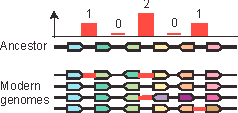
\includegraphics[scale = 2.40]{Ancestor.pdf}
\end{figure}
\end{frame}

\begin{frame}
\frametitle{Intergene Annotation}
CNEs -- conservative non-coding elements
\begin{figure}
	\centering
	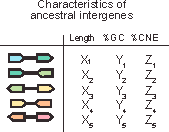
\includegraphics[scale = 2.50]{Annotation.pdf}
\end{figure}
\end{frame}

\begin{frame}
\frametitle{Poisson Regression}
Put intergenes into bins according to predictors:
\begin{enumerate}
\item Intergene length, $L$
\item GC content, \% 
\item Conservative non-coding elements, \%
\end{enumerate}

\vspace{12pt}
Response: breakpoints count / intergene count = or breakage rate $r$
\end{frame}

\begin{frame}
\frametitle{Regression}
Null Hypothesis: pure Poission process

\vspace{12pt}	
Breakpoints are distributed randomly, in direct proportion to
the size of intergenes:

$$r = a \cdot L \Leftrightarrow log(r) = log(L) + \alpha$$

$a$ = average number of breakpoints per intergenic base pair

\pause
\vspace{12pt}
Regression equation:
$$log(r) = \alpha \cdot log(L) + \beta  \cdot \% GC + \gamma  \cdot CNE + \delta$$
or 
$$r = d  \cdot L^\alpha  \cdot e ^ {\beta  \cdot \% GC}  \cdot e ^ {\gamma  \cdot CNE}$$
\end{frame}

\begin{frame}
\frametitle{The Result}
\begin{figure}
	\centering
	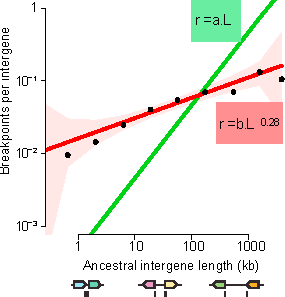
\includegraphics[scale = 1.5]{Plot.pdf}
\end{figure}
\end{frame}

\begin{frame}
\begin{figure}
	\centering
	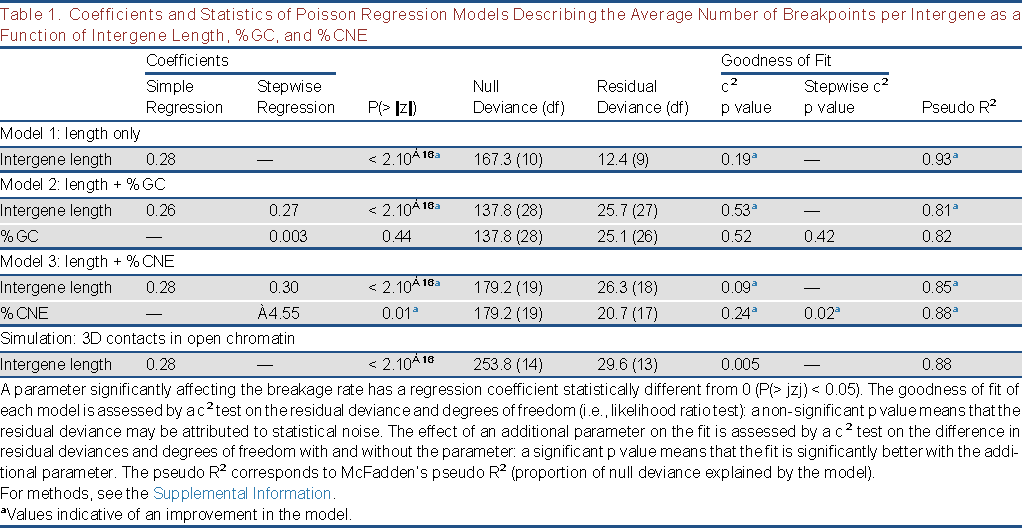
\includegraphics[scale = .67]{Table11.pdf}
\end{figure}
\end{frame}

\begin{frame}
\frametitle{How to Explain the Equation?}
$$r = 2.4 10^{-3} \times L ^ {0.28}$$

Intergene length explains 93\% of variation in breakpoint occurrence
\vspace{12pt}

Short intergenes are more breakable than under pure random model,
while longer ones are less
\vspace{12pt}

Why?
\end{frame}

\begin{frame}
\frametitle{Is GC Content has any Influence?}
GC content strongly correlates with gene density
\vspace{12pt}

Maybe GC content can be a physical explanation?
\pause

\vspace{12pt}
Added GC content in regression --- got a non-significant coefficient
\end{frame}

\begin{frame}
\begin{figure}
	\centering
	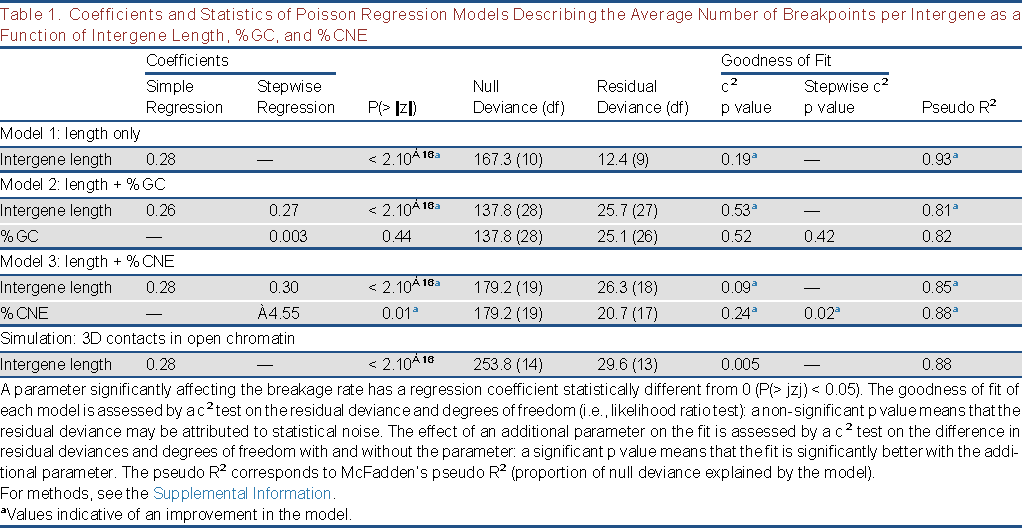
\includegraphics[scale = .67]{Table11.pdf}
\end{figure}
\end{frame}

\begin{frame}
\frametitle{Are CNEs Affect Fragility?}
CNEs -- conservative non-coding elements
\vspace{12pt}

Logic: regulative elements may affect genes that are nearby

\vspace{12pt}
Disrupting synteny between CNEs and genes may have impact on rearrangements that we observe

\vspace{12pt}
Do they?
\vspace{12pt}

\pause
Not that much
\vspace{12pt}

Added CNE rate in regression --- got a significant coefficient, improved explanation rate only by 3\%
\end{frame}

\begin{frame}
\begin{figure}
	\centering
	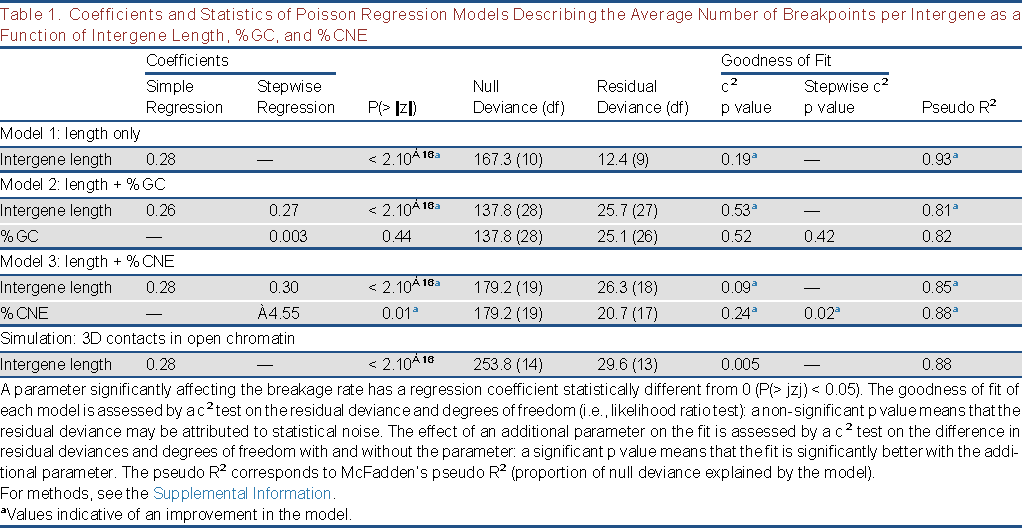
\includegraphics[scale = .67]{Table11.pdf}
\end{figure}
\end{frame}

\begin{frame}
\frametitle{Inversions within Intergenes}
A reminder: we work with gene markers $\Rightarrow$ see only rearrangements disrupting their order
\begin{figure}
	\centering
	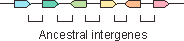
\includegraphics[scale = 2.20]{Intergenes.pdf}
\end{figure}
\vspace{12pt}
Regression showed that longer intergenes have smaller breaks than expected

\vspace{12pt}
What if really missing breakpoints within long intergenes?
\end{frame}

\begin{frame}
\frametitle{Inversions within Intergenes}
Solution: simulate rearrangements, select detectable ones and compare with the real data

\vspace{12pt}
If bias exists, the results should be very close

\vspace{12pt}
Rearrangements have been shown to occur between regions in close 3D proximity in the nucleus

\vspace{12pt}
Contact probability is a good proxy for rearrangement probability
\end{frame}

\begin{frame}
\frametitle{Simulation}
\begin{figure}
	\centering
	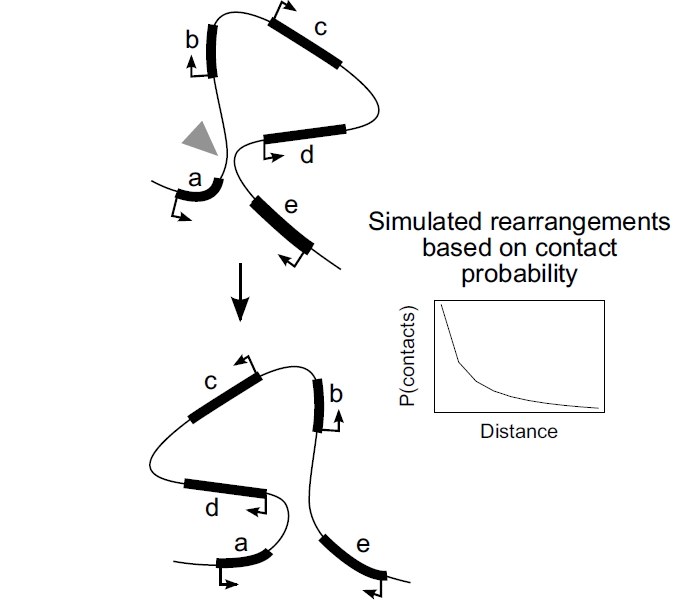
\includegraphics[scale = .40]{Simulation.png}
\caption{Inversions are simulated in the human genome (gray arrow) based on the probability of 3D DNA contacts experimentally derived from Hi-C studies (right inset).}
\end{figure}
\end{frame}

\begin{frame}
\frametitle{Simulation Result}
\begin{figure}
	\centering
	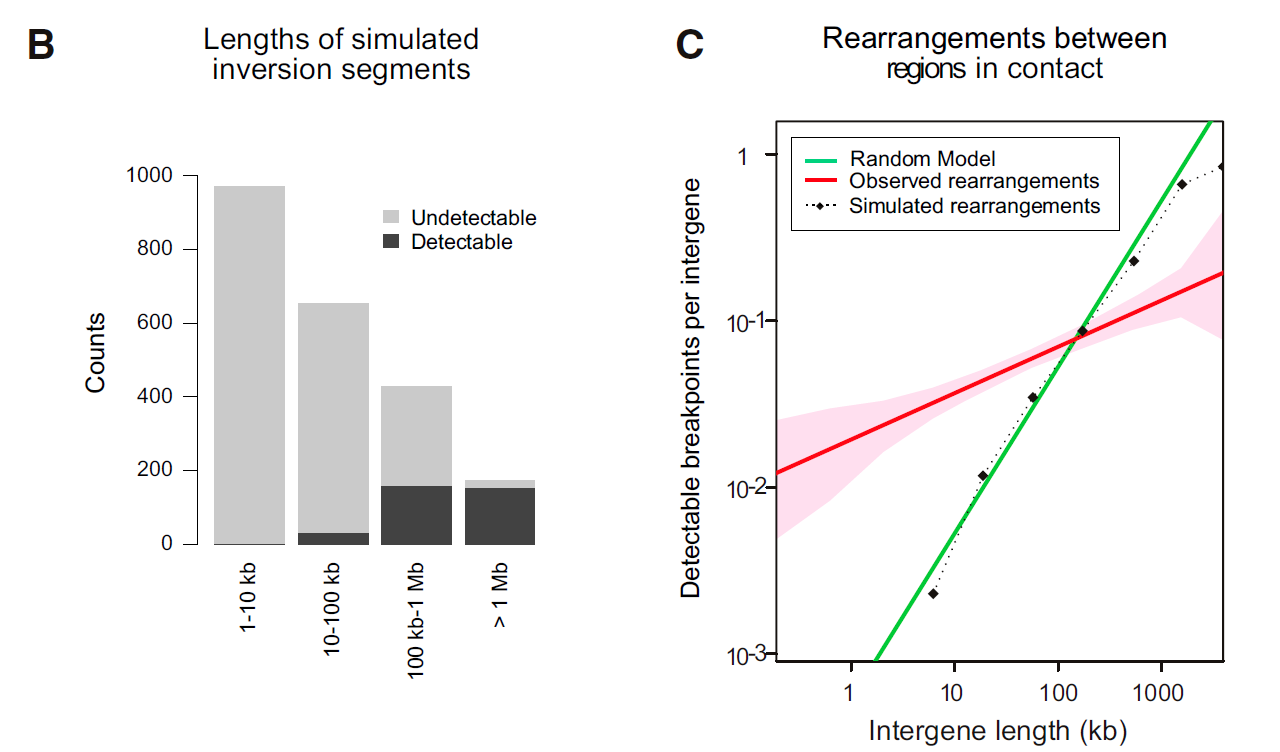
\includegraphics[scale = .31]{SimResult.png}
\end{figure}
Conclusion: non-detected rearrangements do not introduce enough bias
\end{frame}

\begin{frame}
\frametitle{Open Chromatin is the Culprit}
Stick with the simulation -- restrict rearrangements to only \textbf{open chromatin} regions
\vspace{12pt}

ENCODE published chromatin state profiles
\vspace{12pt}

The study used four different cell types
\vspace{12pt}

\pause
Voilà -- simulation coincides with the model!
\end{frame}

\begin{frame}
\frametitle{Simulation Result}
\begin{figure}
	\centering
	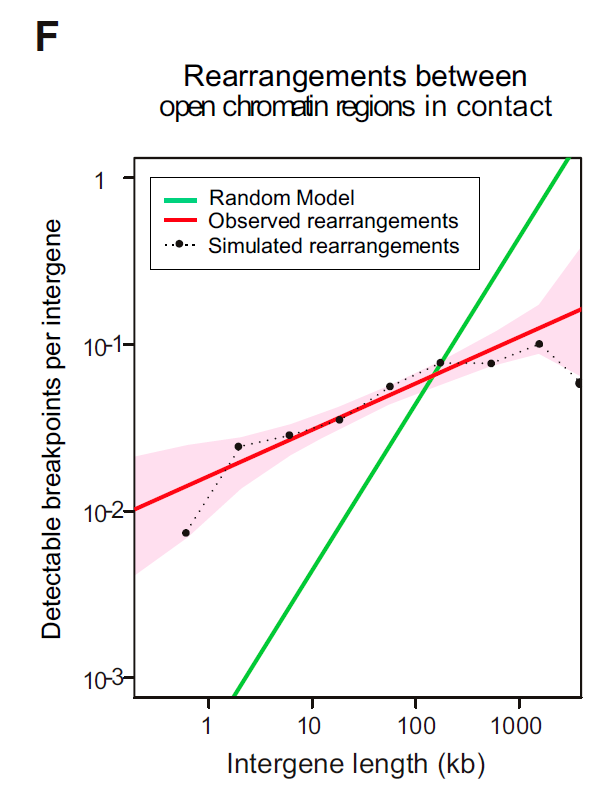
\includegraphics[scale = .38]{SimResult3.png}
\end{figure}
\end{frame}

\begin{frame}
\frametitle{Simulation Result}
\begin{figure}
	\centering
	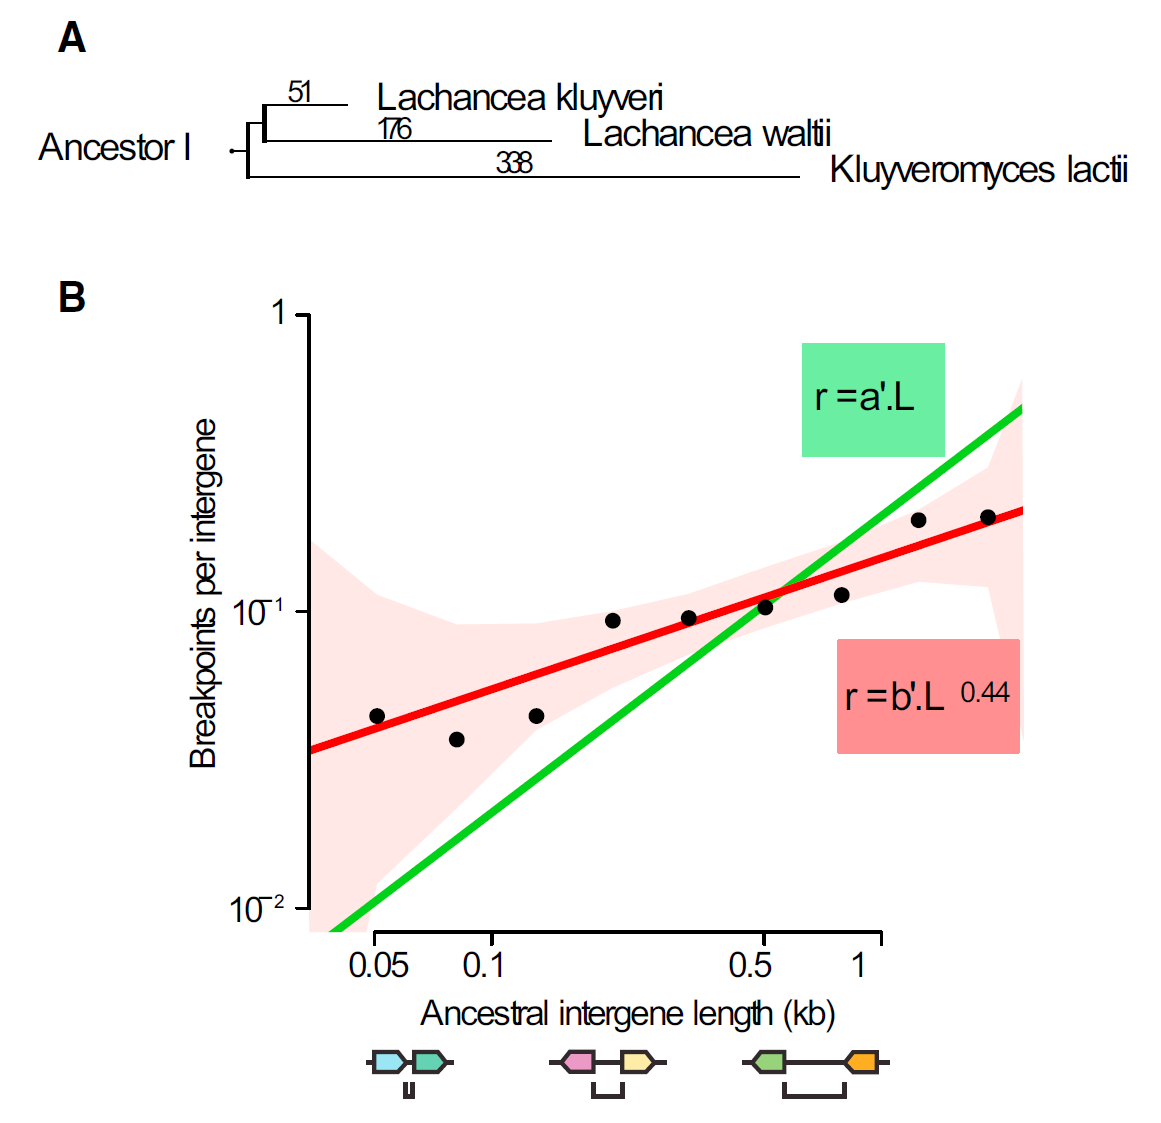
\includegraphics[scale = .3]{Yeasts.png}
\end{figure}
\end{frame}

\begin{frame}
\frametitle{Synteny blocks}
\begin{figure}
	\centering
	\includegraphics[scale = .5]{Synteny.png}
\end{figure}
\end{frame}



\begin{frame}
\frametitle{Conclusion}
A number of interesting insights:
\begin{itemize}
\item Rearrangements are likely to happen in gene dense regions
\item Rearrangement rates depend on location, not content
\item Chromatin state and 3D proximity can be used to predict rearrangements
\item The patterns are consistent in mammals and yeasts
\end{itemize}
\vspace{12pt}

\end{frame}

\begin{frame}
\begin{center}
\hfill \huge \\
Thank you!
\end{center}
\end{frame}


\end{document}
